\begin{td}{Champ électrique dans un conducteur}
\exercice{Effet de peau}
	Le demi-espace $x < 0$ est rempli d'air tandis que le demi-espace
	$x > 0$ est constitué d'un métal. Lorsqu'une onde électromagnétique 
	venant de l'air se réfléchit sur le métal, le métal est le siège de courants
	volumiques de la forme 
	\begin{equation*}
	\vecj = j_0 \exp\left(\dfrac{-x}{\delta}\right)\ey,
	\end{equation*}
	où $j_0$ et $\delta$ sont des constantes.
	\begin{exlist}
		\item Donner la dimension de $j_0$ et de $\delta$. À quoi correspond
		  $\delta$ ?
		\item $\delta$ est appelé l'épaisseur de peau. Elle dépend de
		  la conductivité en régime stationnaire $\sigma$ du matériau considéré
		  et de la pulsation de l'onde électromagnétique $\omega$
		  \begin{equation*}
			  \delta = \sqrt{\dfrac{2}{\mu_0 \omega \sigma}},
		  \end{equation*}
		  où $\mu_0 = \unit{4 \pi \times 10^{-7}}{\kilogram \usk \meter
		  \usk \rpsquare \second \usk \rpsquare \ampere}$ 
		  est la perméabilité magnétique du vide.
		  Vérifier l'homogénéité de cette expression.
		\item Déterminer $\delta$ dans le cas d'un gisement de pyrrhotite
		  de résistivité $\rho = \unit{5 \times 10^{-5}}{\ohm \usk
		  \meter}$ pour 2 méthodes de prospection différentes utilisant des
		  ondes électromagnétiques
		  \begin{exlist}
			  \item induction électromagnétique ($f = \unit{1}{\kilo \hertz}$)
			  \item radar ($f = \unit{100}{\mega \hertz}$)
		 \end{exlist}
		 Ces méthodes permettent-elles de détecter le gisement s'il est enfoui
		 sous un sol de $\unit{3}{\meter}$ d'épaisseur et ayant une résistivité de 
		 $\unit{100}{\ohm \usk \meter}$?
	 	\item L'\oe{}il humain perçoit des ondes électromagnétiques dont la
		  fréquence est située entre $400$ et $\unit{780}{\tera \hertz}$ 
		  environ. Quelle est la valeur de $\delta$ pour ces fréquences et pour
		  le cuivre? Quelle propriété de ce dernier cette valeur traduit-elle ?
	\end{exlist}

\newpage

\exercice{Contamination d'un aquifère}
	De l'eau de mer contamine un aquifère qui sert de source d'eau potable à 
	une ville côtière. Les mesures suivantes de résistivité apparente ont été
	réalisées pour différentes distances inter-électrodes avec la méthode de 
	Wenner pour déterminer la profondeur de la contamination.
	
	\begin{equation*}
	\begin{array}{l l| l l| l l} \\
		a (\meter) & \rho (\ohm \usk \meter) & a (\meter) & 
		\rho (\ohm \usk \meter) &a(\meter) & \rho (\ohm \usk \meter) \\ \hline
		10	& 29.0	& 140	& 19.8	& 280	& 8.7 \\
		20	& 28.9	& 160	& 18.0	& 300	& 7.8 \\
		40 	& 28.5	& 180	& 16.3	& 320	& 7.1 \\
		60	& 27.1  & 200	& 14.5	& 340	& 6.7 \\
		80	& 25.3	& 220	& 12.9	& 360	& 6.5 \\
		100	& 23.5	& 240	& 11.3	& 400	& 6.4 \\
		120	& 21.7	& 260	& 9.9	& 440	& 6.4 \\
	\end{array}
	\end{equation*}
	
	\begin{exlist}
		\item Tracer l'évolution de la résistivité apparente $\rho$ 
		  en fonction de la distance inter-électrode.
		\item Combien de couches différentes pouvez-vous identifier 
		  grâce à cette courbe ? Quelle est leur résistivité respective? 
		  À quelle couche correspond à l'eau salée ?
	  \item Identifier la courbe de résistivité apparente de la figure~\ref{fig:aquiferes}
	    qui correspond au problème. Tracer la résistivité apparente 
	    normalisée par la résistivité de la première 
	    couche en fonction de la distance inter-électrode normalisée pour 
	    différentes valeurs de $d$.
	    Estimer la profondeur de l'interface 
	    aquifère-eau salée. 	
	    \end{exlist}



\begin{figure}[h!]
	\centering
	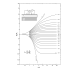
\includegraphics[scale=1.3]{aquiferes}
	\caption{Courbes caractéristiques de résistivité apparente normalisée pour un sol
		 bicouche en fonction de la distance relative inter-électrode 
		 pour le montage de Wenner. Les
	 	notations sont précisées dans la figure. L'image est extraite de 
		\cite{Lowrie2007}}%
	\label{fig:aquiferes}
\end{figure}

\exercice{Le condensateur plan}
On considère un condensateur plan composé de deux plaques conductrices infinies,
parallèles et séparées par une distance $a$. La
première plaque est chargée positivement avec une densité surfacique de charge
$\sigma$, tandis que la deuxième est chargée négativement avec une densité 
surfacique de charge $-\sigma$.

On cherche à déterminer le champ électrique généré par les deux plaques chargées.

\begin{exlist}
	\item Réaliser un schéma du système et choisir un repère adapté.
	\item Quelle est la direction et le sens du champ électrique en un point
	  situé à l'intérieur des deux plaques ?
	\item Étudier les symétries et les invariances du système. 
	\item En appliquant le théorème de Gauss aux trois surfaces suivantes,
	  	  	\begin{exlist}
			\item un cube de section $S$ inclus entre les deux plaques 
			  et situé entre les abscisses $a_1$ et $a_2$,
			\item un cube de section $S$ à l'extérieur des deux plaques
			  entre les abscisses $b_1$ et $b_2$,
			\item un cube de section $S$ contenant une partie 
			  de la plaque $1$ situé entre les abscisses $c_1$ et
			  $c_2$,

		\end{exlist}
	déterminer l'expression du champ électrique généré par les deux plaques
	en tout point de l'espace.
\end{exlist}
\end{td}


